% Graph Attention Network - Mecanismo de atención en grafos
% Compilar con: pdflatex gat_mechanism.tex
\documentclass[tikz,border=10pt]{standalone}
\usepackage{tikz}
\usepackage{amsmath,amssymb}
\usetikzlibrary{arrows.meta, positioning, calc, decorations.markings}

\definecolor{gdlblue}{RGB}{41, 98, 168}
\definecolor{gdlred}{RGB}{191, 49, 49}
\definecolor{gdlgreen}{RGB}{30, 130, 76}
\definecolor{gdlorange}{RGB}{217, 130, 30}
\definecolor{gdlpurple}{RGB}{118, 56, 138}
\definecolor{gdlgray}{RGB}{140, 140, 140}
\definecolor{gdlyellow}{RGB}{190, 140, 10}

\begin{document}
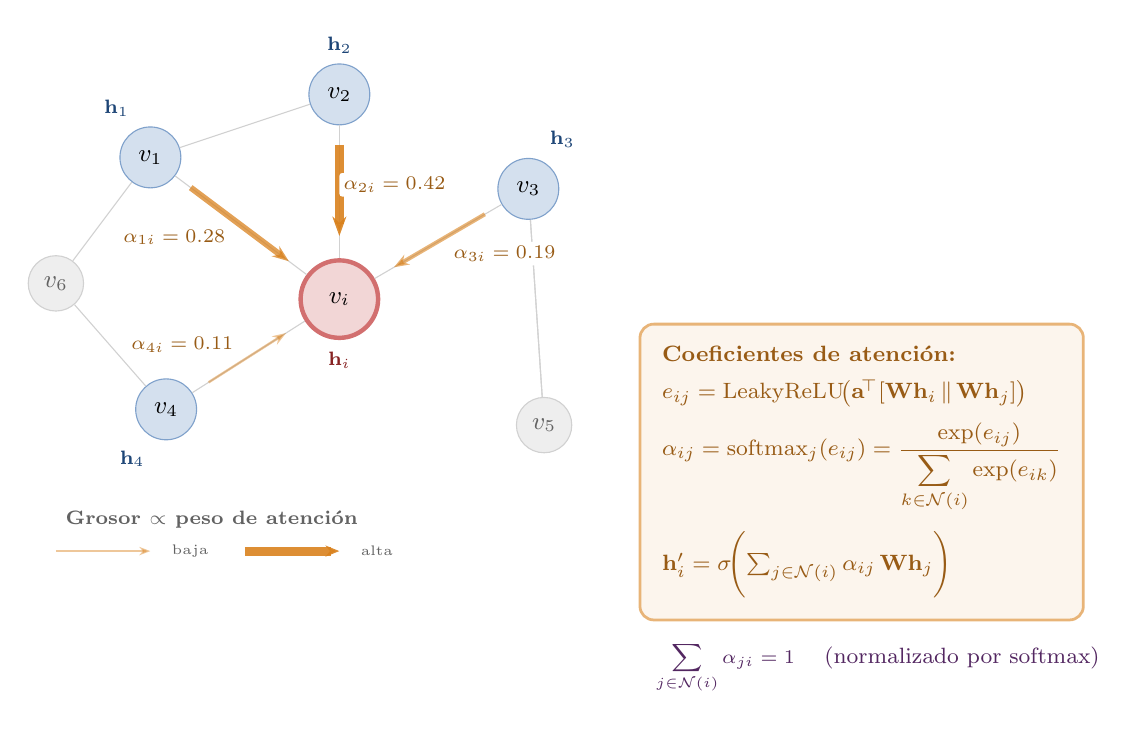
\begin{tikzpicture}[>=Stealth, font=\small]

% ============================================================
% Node styles
% ============================================================
\tikzset{
    targetnode/.style={circle, draw=gdlred!70, fill=gdlred!20,
        minimum size=28pt, inner sep=0pt, font=\small\bfseries,
        line width=1.6pt},
    neighnode/.style={circle, draw=gdlblue!60, fill=gdlblue!20,
        minimum size=22pt, inner sep=0pt, font=\small},
    nonneighnode/.style={circle, draw=gdlgray!40, fill=gdlgray!15,
        minimum size=20pt, inner sep=0pt, font=\small,
        text=gdlgray!70!black}
}

% ============================================================
% Graph structure
% ============================================================

% Central target node
\node[targetnode] (vi) at (0, 0) {$v_i$};

% Neighbor nodes (connected to v_i)
\node[neighnode] (v1) at (-2.4, 1.8)  {$v_1$};
\node[neighnode] (v2) at (0.0, 2.6)   {$v_2$};
\node[neighnode] (v3) at (2.4, 1.4)   {$v_3$};
\node[neighnode] (v4) at (-2.2, -1.4) {$v_4$};

% Non-neighbor nodes
\node[nonneighnode] (v5) at (2.6, -1.6)  {$v_5$};
\node[nonneighnode] (v6) at (-3.6, 0.2)  {$v_6$};

% ============================================================
% Regular (non-attention) edges: gray, thin
% ============================================================
% Edges among non-target nodes
\draw[gdlgray!40, thin] (v1) -- (v6);
\draw[gdlgray!40, thin] (v4) -- (v6);
\draw[gdlgray!40, thin] (v3) -- (v5);
\draw[gdlgray!40, thin] (v1) -- (v2);

% Edges from v_i to neighbors (drawn underneath, as background)
\draw[gdlgray!40, thin] (vi) -- (v1);
\draw[gdlgray!40, thin] (vi) -- (v2);
\draw[gdlgray!40, thin] (vi) -- (v3);
\draw[gdlgray!40, thin] (vi) -- (v4);

% Edge between non-neighbors (no connection to v_i)
\draw[gdlgray!40, thin] (v5) -- (v3);

% ============================================================
% Attention arrows: from neighbors to target node
% Varying line width and opacity to represent attention weights
% ============================================================

% v_2 -> v_i : highest attention (alpha = 0.42)
\draw[-{Stealth[length=7pt,width=5pt]}, line width=3.2pt,
    gdlorange, opacity=0.90, shorten >=8pt, shorten <=7pt]
    (v2) -- (vi);
\node[font=\scriptsize, text=gdlorange!70!black, fill=white,
    inner sep=1.5pt, rounded corners=1pt]
    at ($(v2)!0.48!(vi) + (0.7, 0.1)$) {$\alpha_{2i} = 0.42$};

% v_1 -> v_i : medium-high attention (alpha = 0.28)
\draw[-{Stealth[length=6pt,width=4.5pt]}, line width=2.2pt,
    gdlorange, opacity=0.75, shorten >=8pt, shorten <=7pt]
    (v1) -- (vi);
\node[font=\scriptsize, text=gdlorange!70!black, fill=white,
    inner sep=1.5pt, rounded corners=1pt]
    at ($(v1)!0.48!(vi) + (-0.85, -0.15)$) {$\alpha_{1i} = 0.28$};

% v_3 -> v_i : medium-low attention (alpha = 0.19)
\draw[-{Stealth[length=5.5pt,width=4pt]}, line width=1.5pt,
    gdlorange, opacity=0.60, shorten >=8pt, shorten <=7pt]
    (v3) -- (vi);
\node[font=\scriptsize, text=gdlorange!70!black, fill=white,
    inner sep=1.5pt, rounded corners=1pt]
    at ($(v3)!0.48!(vi) + (0.85, -0.15)$) {$\alpha_{3i} = 0.19$};

% v_4 -> v_i : lowest attention (alpha = 0.11)
\draw[-{Stealth[length=5pt,width=3.5pt]}, line width=0.9pt,
    gdlorange, opacity=0.45, shorten >=8pt, shorten <=7pt]
    (v4) -- (vi);
\node[font=\scriptsize, text=gdlorange!70!black, fill=white,
    inner sep=1.5pt, rounded corners=1pt]
    at ($(v4)!0.48!(vi) + (-0.85, 0.15)$) {$\alpha_{4i} = 0.11$};

% ============================================================
% Feature labels on nodes
% ============================================================
\node[font=\scriptsize, text=gdlred!70!black, anchor=north]
    at ($(vi) + (0, -0.55)$) {$\mathbf{h}_i$};
\node[font=\scriptsize, text=gdlblue!70!black, anchor=south east]
    at ($(v1) + (-0.15, 0.4)$) {$\mathbf{h}_1$};
\node[font=\scriptsize, text=gdlblue!70!black, anchor=south]
    at ($(v2) + (0, 0.4)$) {$\mathbf{h}_2$};
\node[font=\scriptsize, text=gdlblue!70!black, anchor=south west]
    at ($(v3) + (0.15, 0.4)$) {$\mathbf{h}_3$};
\node[font=\scriptsize, text=gdlblue!70!black, anchor=north east]
    at ($(v4) + (-0.15, -0.4)$) {$\mathbf{h}_4$};

% ============================================================
% Annotation: attention computation formula
% ============================================================
\node[rounded corners=5pt, draw=gdlorange!60, fill=gdlorange!8,
    line width=1pt, inner sep=8pt, font=\footnotesize,
    text=gdlorange!70!black, anchor=north west, align=left]
    (formula) at (3.8, -0.3)
    {%
    \textbf{Coeficientes de atenci\'{o}n:}\\[4pt]
    $e_{ij} = \operatorname{LeakyReLU}\!\bigl(
        \mathbf{a}^{\!\top}
        [\mathbf{W}\mathbf{h}_i \,\|\, \mathbf{W}\mathbf{h}_j]
    \bigr)$\\[5pt]
    $\alpha_{ij} = \operatorname{softmax}_j(e_{ij})
    = \dfrac{\exp(e_{ij})}{\displaystyle\sum_{k \in \mathcal{N}(i)} \exp(e_{ik})}$\\[6pt]
    $\mathbf{h}_i^{\prime}
    = \sigma\!\Biggl(
        \sum_{j \in \mathcal{N}(i)} \alpha_{ij}\, \mathbf{W}\mathbf{h}_j
    \Biggr)$
    };

% ============================================================
% Constraint annotation: softmax normalization
% ============================================================
\node[font=\scriptsize, text=gdlpurple!70!black, anchor=north west]
    at ($(formula.south west) + (0.1, -0.15)$)
    {$\displaystyle\sum_{j \in \mathcal{N}(i)} \alpha_{ji} = 1$
    \quad {\footnotesize(normalizado por softmax)}};

% ============================================================
% Visual legend
% ============================================================
\begin{scope}[shift={(-3.6, -2.8)}]
    \node[font=\scriptsize\bfseries, text=gdlgray!70!black, anchor=west]
        at (0, 0) {Grosor $\propto$ peso de atenci\'{o}n};
    % Thin line sample
    \draw[-{Stealth[length=4pt,width=3pt]}, line width=0.9pt,
        gdlorange, opacity=0.45] (0, -0.4) -- (1.2, -0.4);
    \node[font=\tiny, text=gdlgray!70!black, anchor=west]
        at (1.35, -0.4) {baja};
    % Thick line sample
    \draw[-{Stealth[length=5pt,width=4pt]}, line width=3.2pt,
        gdlorange, opacity=0.90] (2.4, -0.4) -- (3.6, -0.4);
    \node[font=\tiny, text=gdlgray!70!black, anchor=west]
        at (3.75, -0.4) {alta};
\end{scope}

\end{tikzpicture}
\end{document}
